\documentclass{article}
% packages and main settings
\usepackage[left=3cm, right=2cm, top=2cm, bottom=2cm]{geometry}
\usepackage[english]{babel}
\usepackage[utf8]{inputenc}
\usepackage[T1]{fontenc}
\usepackage{lmodern}
\usepackage{microtype}
\usepackage{amsmath}
\usepackage{amsfonts, amsthm, amssymb, graphicx, booktabs}
\usepackage{bm} %bold epsilon
\usepackage{newclude}
\usepackage{placeins}  %surpresses floating tables
\usepackage[labelfont=bf]{caption} %Figure etc steht dann in small caps
\usepackage[labelsep=period]{caption} % dot after figure, table caption.
\usepackage[flushleft]{threeparttable} % for notes below table
\usepackage{multirow} % for table cell merge along rows
\usepackage{graphicx} % to adjust tablesize to textwidth
\usepackage{caption}  % for centered captions
\usepackage{float} % to set of autopositioning of tables
\usepackage[bottom,hang,flushmargin]{footmisc} % forces footnotes to the bottom
\usepackage{setspace}           % Fuer 1.5 fachen Zeilenabstand
\onehalfspacing % 1.5 cm Zeilenabstand
%Bibtex
% \usepackage[round,sort&compress]{natbib}

% \bibliographystyle{chicago} % chicago bib style like in AER
\usepackage[hidelinks]{hyperref} % fuer links und verweise. Cleverref ist eigentlich besser.

\usepackage[natbibapa,nodoi]{apacite}

% Create header. The header must be surpressed for
% every first page per section and a solution
% for the Appendix is used in the respective subfile.
\usepackage{fancyhdr}
\pagestyle{fancy}
\fancyhf{}
\chead{\nouppercase{\textit{\leftmark}}}
\cfoot{\thepage}
\renewcommand{\headrulewidth}{0pt} % no vertical line
\usepackage{enumerate}


%\usepackage{lipsum}  % check if formats work

\usepackage{afterpage} %clearpage w/o pagebreak for "header bug"

% Expectation symbol
\DeclareMathOperator*{\E}{\mathbb{E}}

 % thin space, limits underneath in displays
% for strike through
\DeclareMathOperator*{\argmax}{argmax}
\newcommand*{\defeq}{\stackrel{\text{def}}{=}}
\usepackage[normalem]{ulem}
% try to use strikeout in section headers and others
\DeclareRobustCommand{\hsout}[1]{\texorpdfstring{\sout{#1}}{#1}}

% for gray table row color
\usepackage[table]{xcolor}

% decimal dot alignment in table columns
\usepackage{siunitx}

% for footnotes in table
\usepackage[flushleft]{threeparttable}

% for underbar
\newcommand{\ubar}[1]{\text{\b{$#1$}}}

\usepackage{tikz}

% Setup for urls
\usepackage{url}


%Steps list
\usepackage{enumitem}

\usepackage{caption}

\title{QBSM}
\author{liyulei2018 }
\date{September 2021}

\begin{document}

\begin{titlepage}

\begin{center}

\vspace*{1.0cm}

{\LARGE
\bfseries Quantile-based Sensitivity Analysis \\
\vspace*{0.5cm}
on Structural Behavioral Models
}


{\large
\vspace*{4.0cm}
Master Thesis Presented to the\\
\vspace*{0.25cm}
Department of Economics at the\\
\vspace*{0.25cm}
Rheinische Friedrich-Wilhelms-Universität Bonn\\

\vspace*{2.0cm}
in Partial Fulfillment of the Requirements for the Degree of\\
\vspace*{0.25cm}
Master of Science (M.Sc.)\\

\vspace*{4.0cm}
Supervisor: Prof. Dr. Philipp Eisenhauer\\

\vspace*{2.0cm}
Submitted in September 2021 by:\\
Yulei Li\\
Matriculation Number: 3209294
}

\end{center}

\end{titlepage}

\newpage

\thispagestyle{plain} % no header on first page
\tableofcontents
\newpage


\setcounter{page}{1}
\pagenumbering{Roman}



% no section command to prevent "A" before "Appendix" in toc.

\addcontentsline{toc}{section}{Abbreviations}

\section*{Abbreviations} % no number before Appendix in toc
\thispagestyle{plain} % surpress header on first page

\phantom{This text will be invisible}
\hspace{20cm}



% Please add the following required packages to your document preamble:
% \usepackage{booktabs}
\begin{table}[H]
	\centering
	\renewcommand{\arraystretch}{1.2}%
	\begin{tabular}{@{}ll@{}}
		\toprule
	Term\phantom{space}	& Meaning \\ \midrule
	$\bold{CDF}$	& Cumulative distribution function \\
	$\bold{DCDP}$	& Discrete choice dynamic programming  \\
	$\bold{EKW}$	& Eckstein-Keane-Wolpin  \\
	$\bold{GSA}$	& Global sensitivity analysis \\
	$\bold{LSA}$	& Local sensitivity analysis \\
	$\bold{PDF}$	& Probability distribution function \\
	$\bold{QBSM}$	& Quantile-based sensitivity measures \\
    $\bold{QoI}$	& Quantity of interest \\
    $\bold{USD}$	& US-Dollar  \\
 \bottomrule
	\end{tabular}
\end{table}
\newpage


\addcontentsline{toc}{section}{List of Figures}

%\section*{List of Figures} % no number before LoFs in toc
\thispagestyle{plain} % surpress header on first page

\listoffigures
\newpage


\addcontentsline{toc}{section}{List of Tables}

%\section*{List of Tables} % no number before LoTs in toc
\thispagestyle{plain} % surpress header on first page

\listoftables
\newpage


\setcounter{page}{1}
\pagenumbering{arabic}

\section{Introduction}
\thispagestyle{plain} % surpress header on first page

Structural econometric models have been widely used to provide decision support and guidelines for policymakers. The Discrete Choice Dynamic Programming (DCDP) model, a structural model commonly used in the field of labor economics, plays a key role in evaluating the effects of various policy interventions. In particular, DCDP models study schooling and occupational choice and investigate the effects of policy interventions designed to boost human capital investment, such as parental and government subsidies and student loan programs \citep{keane1997CareerDecisionsYoung, sauer2004EducationalFinancingLifetime}.\\

\noindent
A typical structural model of optimal individual behavior consists of a number of structural parameters that capture the underlying preferences and constraints of the individual’s decision process \citep{blundell2017WhatHaveWe}. Such models require individuals to solve a sequential decision problem under given institutional constraints that are determined by a set of variables determined by policymakers (e.g., tax rates). So far, most structural models have been deterministic, with each model parameter fixed with a single numerical value or point estimate, ignoring their associated errors or uncertainties. \citep{adda2017CareerCostsChildren, attanasio2012EducationChoicesMexico, eckstein2019CareerFamilyDecisions}. In addition to using point estimates, policymakers can obtain more information about prediction errors by including uncertainty in the model parameters. For example, using confidence sets as set estimates \citep{manski2021EconometricsDecisionMaking}. More recently, noticing the considerable parametric uncertainty in prediction, \cite{eisenhauer2021StructuralModelsPolicymaking} suggested the use of global sensitivity analysis to identify which parameters are particularly responsive to prediction uncertainty.\\

\noindent
Sensitivity analysis(SA) has been a well-established approach in a wide variety of scientific disciplines, such as biology \citep{zi2011SensitivityAnalysisApproaches}, chemistry \citep{saltelli2005SensitivityAnalysisChemical}, environmental sciences \citep{campolongo1997SensitivityAnalysisEnvironmental} and so on. However, economists have had a very restricted contribution to the literature on sensitivity analysis. Although the importance of sensitivity analysis for quantitative models has been well acknowledged by some economists, very few studies have included any form of sensitivity analysis when building economic models, or if they do, they often rely on local techniques, in which case the sensitivity measures are only computed around a fixed point in the parameter space \citep{canova1994StatisticalInferenceCalibrated, harenberg2019UncertaintyQuantificationGlobal, leamer1985SensitivityAnalysesWould}. It is notable that SA in economics research is distinguished from other areas such as environmental science by the conditional distribution of the input parameters. As a result, using a one-factor-at-a-time Local SA without accounting for any parameter correlations would yield misleading results. Moreover, Local methods have the glaring drawback that they are invalid for nonlinear and nonmonotonic models \citep{saltelli2004SensitivityAnalysisPractice}, which are frequently used in econometric modeling. In contrast, global methods with a “model-free” setting are strongly recommended in systematic reviews \citep{saltelli2019WhyManyPublished}. Unfortunately, a generally accepted practice of GSA has not yet been established in most of the existing economic literature.\\

\noindent
I rely on quantile-based sensitivity measures(QBSM) \citep{kucherenko2019QuantileBasedGlobal} to analyze the impact of the parametric uncertainty on prediction uncertainty. Such measures are based on quantiles of the model output, which allow us to identify the parametric uncertainty at quantile level. The quantiles of output Cumulative distribution(CDF) are also of interest in other domains such as reliability analysis and financial risk analysis. For such problems, conventional method such as variance-based sensitivity indices \citep{sobol1993SensitivityEstimatesNonlinear} are in practical. Moreover, variance-based sensitivity measures are not able to identify variables that are most essential in achieving the extreme values of the model output. Alternatively, QBSM are designed for global sensitivity analysis of problems where the $\alpha$-th quantile is a function of interest, and also for instances where the analyst is interested in the ranking of the inputs that cause the extreme values of the output. The quantile oriented sensitivity indices \citep{kala2019QuantileorientedGlobalSensitivity} share some similarities with QBSM, but these indices are based on contrast function instead of explicitly depending on quantiles.\\

\noindent
As an application, I reanalyze the human capital investment decision model by \cite{keane1994SolutionEstimationDiscrete}. I estimate the model parameters and replicated the key results using the provided dataset. I generate counterfactual predictions based on the estimated parameters.  I investigate the transition of uncertainty from key parameters to model output. I calculate the QBSM for a few parameters to identify the parameters that contribute most to the prediction uncertainty.  I extend their framework to explain which parameter specifically contributes to the uncertainty. \\

\noindent
This work complements the work by \cite{eisenhauer2021StructuralModelsPolicymaking}, who documented significant prediction uncertainty in a Eckstein-Keane-Wolpin(EKW) model \citep{aguirregabiria2010DynamicDiscreteChoice}. My work builds on their work by identifying which parameters account for most of the output uncertainty based on the quaniles of output. In their study, a 90\% confidence set is used to represent the counterfactual uncertainty. As a result, the analyst is primarily concerned with the region of the output values range inside the confidence set. In other words, the critical quantiles of the cumulative distribution function (CDF) of the function are of interest, which fits well with the target problem that QBSM aim to addresses. Although including sensitivity analysis in model calibration has long been a standard technique in environmental and engineering modeling, there is a lack of application in econometric modelling.\\


\noindent
This paper is organized as follows: Section \ref{sec:2} presents the model setting of \cite{keane1994SolutionEstimationDiscrete}. Section \ref{sec:3} gives an introduction to variance-based global sensitivity indices and QGSM. Algorithms and methods for numerical estimation of QGSM are discussed in Section \ref{sec:3}. The results are presented in Section \ref{sec:5}.  Finally, conclusions are summarized in Section \ref{sec:6}.\\


\section{The Structural Behavioral Model} \label{sec:2}
\thispagestyle{plain} % surpress header on first page


The SA approach is applied to the DCDP model of the human capital investment decisions presented in \cite{keane1994SolutionEstimationDiscrete} which is briefly described in subsection \ref{sec:2.1}. The uncertain input parameters of the model are described in subsection \ref{sec:2.2} and the quantity of interest is discussed in subsection \ref{sec:2.3}.

\subsection{\cite{keane1994SolutionEstimationDiscrete} model} \label{sec:2.1}

Structural models have been developed to understand individual behavior and inform policy design in labor economics, particularly for DCDP models. DCDP models, as a framework for policy evaluation, have been applied to study a range of sequential individual decisions. A notable example is a work by \cite{keane1994SolutionEstimationDiscrete}, who developed an approximate solution to a large-scale DCDP model of human capital occupational choice. This is an ideal demonstration of how a structural model can evaluate various policies and determine the optimal policy without running many treatments.\\

\noindent
We assume that individuals are forward looking agents who make their occupational choice based on the principle of expected utility maximization. From age 15 to the age 55, the total period of decision is $T=40$ years. As shown in Figure \ref{fig:1}, in each period $t$, individual makes choice among $K=4$ alternatives: occupation one($a_t=1$), occupation two($a_t=2$), schooling($a_t=3$) and staying at home($a_t=4$). We denote the agent's immediate rewards of choosing each alternative in a given period as:


\begin{equation}
r_{t}\left(s_{t}, a_{t}\right)=\left\{\begin{array}{ll}
w_{1 t}=\exp \left\{\alpha_{10}+\alpha_{11} g_{t}+\alpha_{12} e_{1 t}+\alpha_{13} e_{1 t}^{2}+\alpha_{14} e_{2 t}+\alpha_{15} e_{2 t}^{2}+\epsilon_{1 t}\right\} & \text { if } a_{t}=1 \\
w_{2 t}=\exp \left\{\alpha_{20}+\alpha_{21} g_{t}+\alpha_{22} e_{1 t}+\alpha_{23} e_{1 t}^{2}+\alpha_{24} e_{2 t}+\alpha_{25} e_{2 t}^{2}+\epsilon_{2 t}\right\} & \text { if } a_{t}=2 \\
\beta_{0}-\beta_{1} \mathbb{I}\left[g_{t} \geq 12\right]-\beta_{2} \mathbb{I}\left[a_{t-1} \neq 3\right]+\epsilon_{3 t} & \text { if } a_{t}=3 \\
\gamma_{0}+\epsilon_{4 t} & \text { if } a_{t}=4
\end{array}\right.
\end{equation}
$w_{1t}$ and $w_{2t}$ is occupational-specific wage if individual choose either occupation one or two. $\alpha_1$ and $\alpha_1$ are parameters of corresponding wage functions. The primary factors that associated to wages are: years of completed schooling($g_t$), years of working experience in two occupations respectively($e_{1t}$, $e_{2t}$).If the individual does not choose to work($a_t=3$ or $a_4 = 4$), although they are not paid during this period, they still receive rewards from their choices. The variables that influence the choice of schooling are: the consumption value of schooling($\beta_0$), the tuition of post-secondary education($\beta_1$), and the adjustment expenses involved with returning to school. The means return of staying at home that affects the home option is represented by $\gamma_0$. \\

\noindent
The state space $t$ can be represented by
\begin{equation} \label{eq:2}
\left\{g_{t}, e_{1 t}, e_{2 t}, a_{t-1}, \epsilon_{1 t}, \epsilon_{2 t}, \epsilon_{3 t}, \epsilon_{4 t}\right\}
\end{equation}



\noindent
The part of state space observable to both individuals and researchers are $\left\{g_{t}, e_{1 t}, e_{2 t}, a_{t-1}\right\}$. The evolution of those variables follows a Markov chain, which means that the next state at period $t+1$ relies on the current state $t$ and the decision maker's action:


\begin{equation}\label{eq:3}
\begin{aligned}
e_{1, t+1} &=e_{1 t}+\mathbb{I}\left[a_{t}=1\right] \\
e_{2, t+1} &=e_{2 t}+\mathbb{I}\left[a_{t}=2\right] \\
g_{t+1} &=g_{t}+\mathbb{I}\left[a_{t}=3 \right]
\end{aligned}
\end{equation}
The shocks$\{\epsilon_{1t}, \epsilon_{2t},, \epsilon_{3t}, \epsilon_{4t}\}$ are serially independent and observed by individuals but not researchers.They are assumed to be jointly normally distributed. \\

\noindent
The maximized value of the expected remaining lifetime utility at $t$ is defined as:

\begin{equation}\label{eq:4}
V(S(t), t)=\max _{\left\{d_{k}(t)\right\}_{k \in K}} E\left[\sum_{\tau=t}^{T} \delta^{\tau-t} \sum_{k=1}^{K} R_{k}(\tau) d_{k}(\tau) \mid S(t)\right]
\end{equation}
with $0< \beta < 1$ the discount factor. $S(t)$ are state variables that contain information available before decision in period $t$ is made. $R_k$ is the rewards from choose alternative $k$ at period $t$. $d_k$ is individual's decision from among K=4 discrete alternatives. \\

\noindent
Alternatively, this optimization problem can be expressed as a the Bellman equation, which is a necessary condition for optimality associated with dynamic programming\citep{bellman1966DynamicProgramming, eisenhauer2019ApproximateSolutionFinite}:

\begin{equation}
E \max (S(t+1))=E\left[V(S(t+1), t+1) \mid S(t), d_{k}(t)=1\right]
\end{equation}



\subsection{Model parameters} \label{sec:2.2}



For model parametrization, our work takes advantage of the open-source Python package respy\citep{janosgabler2020RespyFrameworkSimulation}, which has greatly simplified the process of simulation and estimation of finite-horizon DCDP models. Table \ref{tab:1} shows the parameter values obtained from the simulation based on Data Set One in \cite{keane1994SolutionEstimationDiscrete}. According to this setting, occupation two requires greater expertise and thus is more beneficial from education. Experience in occupation one also increases the likelihood of increased earnings in another occupation. Thus, a general skill that is useful for both occupations can be obtained through either schooling or work experience, while occupation-specific skills are exclusively obtained through work. In this sense, we will refer to occupation two as white-collar and occupation one as blue-collar henceforth. \\

\noindent
Once parameterization is completed, we are allowed to analyze the economic implications behind it. Firstly, we investigate the correlation between selective model parameters \ref{fig:3}. In general, a large share correlation are prevalent, which emphasizes the importance of using GSA rather than LSA for this model. Because GSA takes into account the interaction between parameters. It is also worth noting that $\hat{\delta}$ and $\hat{\beta_0}$ and beta show a relatively strong negative correlation. \\


\noindent
\subsection{Quantity of Interest(QoI)} \label{sec:2.3}


This paper measures the impact of a 500 USD tuition subsidy on the average number of years a individual spends on pursuing a higher education degree. Figure \ref{fig:2} shows the probability distribution of this quantity of interest. Our simulation results with respy\citep{janosgabler2020RespyFrameworkSimulation} showed a 1.55-year increase in average school years, which is slightly higher than the effect documented by \cite{keane1994SolutionEstimationDiscrete}, that is an increase of 1.44 years. More specifically, Figure \ref{fig:3} shows a comparison of the occupation shares over their relevant life cycle for a sample of 1000 individuals in different sectors. The left panel shows a baseline scenario that without any policy intervention, whereas the right panel shows a counterfactual scenario that all the 500 USD tuition subsidy is implemented. The yellow, green, dark blue and light blue bars represent the percentages of people stay-at-home, pursuing education, blue-collar, white-collar, respectively. With this setting, we are able to access the policy effect without running experiments at real world. \\

\noindent
We noticed the change that, due to the fact that the white-collar industry values education, many agents begin their schooling early and continue to work in the white-collar sector. The positive impact and accumulated blue-collar experience pays off in the white-collar sector as well, leading to this shift from white- to blue-collar. It is nearly on impact due to the overall low level of participation in the household sector. The difference between the education shares for each age group in the right and left graphs, as represented by the red line, is quantified investment. This is because the vertical axis can be thought of as the percentage of time a typical agent spends in the education sector over the course of a year. When we look at both graphs, we can clearly see that tuition subsidies encourage younger people to stay in school longer and older people to pursue white collar works.\\


\noindent
In section \ref{sec:3} and section for \ref{sec:4} I will present how uncertain in model input translate to the variations of model output, in this case, the average change of school years. However, due to the computational burden in the sampling procedure, I restrict my attention to three main parameters: return to an additional year of schooling$\alpha_{11}$, reward for going to college$\beta_1$ and reward of non-market alternatives$\gamma_0$. As what we study is the impact of subsidy, the profit/cost trade-offs involved with the decision whether to pursue continuing education are fully reflected by the return on educational investment. Although $\gamma_0$ seems not explicitly related to our QoI like the previous chosen ones, we include is as a comparison.


\section{Sensitivity Analysis for the Structural Behavioral Model} \label{sec:3}
\thispagestyle{plain} % surpress header on first page


In this chapter, we introduce the basic concepts, terminologies, methods of GSA in Section \ref{sec:3.1}, including the general model structure and the input factors. Then we demonstrate the mathematical descriptions of the variance-based and quantile-based sensitivity measures in Section \ref{sec:3.2} and Section \ref{sec:3.3}.

\subsection{Global sensitivity analysis: the framework} \label{sec:3.1}

The sensitivity analysis is “The study of how the uncertainty in the output of a model (numerical or otherwise) can be apportioned to different sources of uncertainty in the model input”\citep{saltelli2004SensitivityAnalysisPractice}. Thus, the definition of sensitivity analysis includes models, model inputs and model outputs. Throughout this work, a structural economic model will be regarded as a general function that defines a relationship between inputs and output(s):

\begin{equation} \label{eq:6}
\mathcal{M}: \theta \mapsto y=\mathcal{M}(\theta)
\end{equation}


\noindent
where $\boldsymbol{\theta} \in \Theta \subset \mathbb{R}^{d}$ is a vector of model parameters. The output of interest is a vector $y$. To produce a counterfactual prediction, a policy $g \in \mathcal{G}$ changes the mapping to $\mathcal{M}_g(\theta)$\citep{eisenhauer2021StructuralModelsPolicymaking}. Consequently, the differences between the prediction before and after the policy intervention yield a structural estimate of policy effects. \\

\noindent
Unlike LSA which analyzes how a tiny change near an input space value affects the scalar output, GSA identifies such effects in the whole input space. To be more precise, each input parameter is treated as a random variable assigned with a distribution of all possible values. Consequently, the uncertainty coming from model parameters is transmitted through the model to generate an empirical distribution of the output of interest $Y = M(\Theta)$ with a joint probability density function $f_Y(y)$. So far, this is how uncertainty propagation occurs. \\

\noindent
Once uncertainty propagation characterizes the uncertainty of the model output, a sensitivity analysis then can be applied to identify which parameters are primarily responsible for the variability of output. \\

\noindent
To date, a wide range of GSA methods has been developed. In this paper, we focus on variance-based sensitivity measures\citep{sobol1993SensitivityEstimatesNonlinear} and quantile-based sensitivity measures\citep{kucherenko2019QuantileBasedGlobal}. A comprehensive discussion and comparison of the GSA methods can be found in \cite{razavi2021FutureSensitivityAnalysis}.

\subsection{Variance-based sensitivity measures}  \label{sec:3.2}

The model function $Y=f\left(\theta_{1}, \ldots, \theta_{d}\right)$ is defined in $d$-dimensional real coordinate space $R^d$ with an input vector $\boldsymbol{\theta}=(\theta_1, \dots, \theta_{d})$.Note that $\mathbf{\theta}$ is a random variable with a continuous probability distribution function(PDF). To quantify the effect of variations of $\theta$ on the variation of $Y$, let us consider the conditional expectation  $\mathrm{E}\left[Y \mid \Theta_{i}=\theta_{i}\right]$. It is the mean value of output $Y$ over the probability distribution of  $\Theta_k(k \neq i)$ with the condition that $\Theta_i$ is fixed to $\theta_i$. If we consider the variations of $\Theta_i$,  the associated random variable is  $\mathrm{E}\left[Y \mid \Theta_{i}\right]$, whose variance quantifies the effect of $\Theta_i$ on the variation of Y. \\

\noindent
According to the result by \cite{sobol1993SensitivityEstimatesNonlinear}, given $k$ input variables mutually independent, the variance of the output can be decompose as the sum of variances of increasing order:

\begin{equation} \label{eq:7}
\operatorname{Var}(Y)=\sum_{i} V_{i}+\sum_{i j} V_{i j}+\sum_{i j h} V_{i j k}+\cdots+V_{1,2}, k
\end{equation}

\noindent
where $V_i = \operatorname{Var}(E(Y \mid \Theta_i))$ is first order variance and $V_{ij} = \operatorname{Var}(E(Y \mid \Theta_i,\Theta_j))$ is second order variance, etc. Note that in an additive model, this decomposition includes only first order variances. \\

\noindent
Thus, \textit{first-order indice}s of input parameter $\Theta_i$ is defined as:

\begin{equation} \label{eq:8}
S_i = \frac{V_i}{\operatorname{Var}(Y)}=\frac{\operatorname{Var}(E(Y \mid \Theta_i))}{\operatorname{Var}(Y)}
\end{equation}

\noindent
Accordingly, \textit{second-order indices} of input parameter $\Theta_i$ and $\Theta_j$ is defined as:


\begin{equation} \label{eq:9}
S_{ij} = \frac{V_{ij}}{\operatorname{Var}(Y)}=\frac{\operatorname{Var}(E(Y \mid \Theta_i,\Theta_j))}{\operatorname{Var}(Y)}
\end{equation}

\noindent
First-order indices measures the proportion of the total variance which is due to the main effect of $\Theta_i$ on Y. Whereas, second-order index measures the proportion of the total variance which is explained by the interaction between the two inputs. \\

\noindent
In 1996, \cite{homma1996ImportanceMeasuresGlobal} introduced the \textit{total variance index} which measures the proportion of the total variance due to the
main effect of $\Theta$, and all its interactions with the other inputs:

\begin{equation} \label{eq:10}
S_{Ti}=\frac{\sum_{i} V_{i}+\sum_{j h} V_{i j h}+\cdots}{\operatorname{Var}(Y)} = \frac{E(Var(Y \mid \Theta_{\sim i}))}{Var(Y)}=1-\frac{Var(E(Y \mid \Theta _{\sim i})}{Var(Y)}
\end{equation}

\noindent
where $\Theta_{\sim i}=(\Theta_1, \Theta_2, \dots, \Theta_{i-1}, \Theta_{i+1}, \dots ,  \Theta_k)$ \\

\noindent
There are three features of total variance index to be aware of. Firstly, The condition $S_{Ti}=0$ is necessary and sufficient for $\Theta_i$ to be a non-influential input(it can be treated as a fixed input). Secondly, if $S_{Ti} \approx S_i$ the interaction between $\Theta_i$ and the other inputs does not affect the variability of the output. Lastly, it is obvious that the sum of the total indexes is in general greater than \cite{homma1996ImportanceMeasuresGlobal}.


\subsection{Quantile-based sensitivity measures}  \label{sec:3.3}

Now we consider the scenarios where only a specific range of output is important to analyst. For instance, $Y = M(\boldsymbol(\Theta) \leq a )$ or $Y = M(\boldsymbol(\Theta) \geq b$. We reformulate such problems to $\alpha$-th quantile of the output CDF $q_Y(\alpha)$:


\begin{equation} \label{eq:11}
\alpha=\int_{-\infty}^{q_{Y}(\alpha)} \rho_{Y}(y) d y=P\left\{Y \leq q_{Y}(\alpha)\right\}
\end{equation}

\noindent
alternatively, to be more formal:

\begin{equation} \label{eq:12}
q_{Y}(\alpha)=F_{Y}^{-1}(\alpha)=\inf \{y \mid F(Y \leq y) \geq \alpha\}
\end{equation}

\noindent
where $\rho_Y(y)$ denotes the PDF of the output $Y$ and $F_Y(y)$ denotes to the CDF of the output $Y$.To solve such problems, \cite{kucherenko2019QuantileBasedGlobal} introduced QBSM $\bar{q}_{i}^{(1)}$ and $\bar{q}_{i}^{(2)}$

\begin{equation} \label{eq:13}
\bar{q}_{i}^{(1)}(\alpha)=E_{\theta_{i}}\left(\left|q_{Y}(\alpha)-q_{Y \mid \Theta_{i}}(\alpha)\right|\right)=\int\left|q_{Y}(\alpha)-q_{Y \mid \Theta_{i}}(\alpha)\right| d F_{\theta_{i}}
\end{equation}

\begin{equation} \label{eq:14}
\bar{q}_{i}^{(2)}(\alpha)=E_{\theta_{i}}\left[\left(q_{Y}(\alpha)-q_{Y \mid \Theta_{i}}(\alpha)\right)^{2}\right]=\int\left(q_{Y}(\alpha)-q_{Y \mid \Theta_{i}}(\alpha)\right)^{2} d F_{\theta_{i}}
\end{equation}

\noindent
Here,  $F_{\Theta_i}$ denotes to the CDF of input variable, $q_{Y \mid \Theta_{i}}({\alpha})$ denotes to the conditional PDF with $\Theta_{i}$ being fixed at $X_{i}=x_{i}^{\mbox{*}}$ \citep{song2021QuantileSensitivityMeasures}

\begin{equation}\label{eq:15}
q_{Y \mid \Theta_{i}}(\alpha)=F_{Y \mid \Theta_{i}}^{-1}(\alpha)=\inf \left\{P\left(Y \leq y \mid \Theta_{i}=\theta_{i}^{*}\right) \geq \alpha\right\}
\end{equation}


\noindent
Additionally, a normalized version of QBSM $Q_{i}^{(1)}(\alpha)$ and $Q_{i}^{(2)}(\alpha)$ was also presented in \cite{kucherenko2019QuantileBasedGlobal}:

\begin{equation}\label{eq:16}
Q_{i}^{(1)}(\alpha)=\frac{\bar{q}_{i}^{(1)}(\alpha)}{\sum_{j=1}^{d} \bar{q}_{j}^{(1)}(\alpha)}
\end{equation}

\begin{equation}\label{eq:17}
Q_{i}^{(2)}(\alpha)=\frac{\bar{q}_{i}^{(2)}(\alpha)}{\sum_{j=2}^{d} \bar{q}_{j}^{(2)}(\alpha)}
\end{equation}

\noindent
with $\left\{Q_{i}^{(1)}(\alpha), Q_{i}^{(2)}(\alpha)\right\} \in[0,1]$.






\section{Monte Carlo Simulation} \label{sec:4}
\thispagestyle{plain} % surpress header on first page

Because QBSM has no closed-form expression, they must be assessed numerically through Monte Carlo(MC) simulation\citep{fishman1996MonteCarloConcepts}. MC simulation generates random samples from a probability distribution, and the problem becomes deterministic for each sample. Solving these deterministic problems allows us to obtain statistical information regarding the exact solutions, such as the mean or variance. However, MC approaches are renowned for their slow convergence, with an average coverage rate of $\sqrt N$(N stands for the sample size). This means that, to get more precise outcomes, a large number of samples are required.
Although various improved MC methods have been developed, such as Latin sampling methods\citep{loh1996LatinHypercubeSampling} and Quasi-Monte Carlo(QMC) methods\citep{niederreiter1992RandomNumberGeneration}, there are still certain limits to it. \\

\noindent
In \cite{kucherenko2017DifferentNumericalEstimators}, the performance of several numerical schemes based on sampling strategies was compared. It is documented that the double loop reordering(DLR) technique outperforms all other methods, especially when combined with QMC sampling. In this paper, by integrating the two MC estimators provided by \cite{kucherenko2019QuantileBasedGlobal} and the procedure improved by \cite{song2021QuantileSensitivityMeasures}, we list the following steps to estimate QBSM in our study:

\begin{itemize}
\item \textbf{Step 1:} To obtain  $q_{Y \mid \Theta_{i}}$:

\begin{enumerate}[label=(\arabic*),ref=\arabic*]
  \item Generate $N$ points  $\boldsymbol{\Theta}^{(k)}=\left\{\Theta_{1}^{(k)}, \Theta_{2}^{(k)}, \cdots, \Theta_{d}^{(k)}\right\}, k=1,2, \cdots, N$ according to the joint PDF $ \rho (\boldsymbol{\Theta)}$.


  \item Compute the unconditional values of output $Y^{(k)}=g\left(\boldsymbol{\Theta}^{(k)}\right), k=1, 2, \dots, N$, then reorder them in ascending order $\left\{Y^{(1-s t)}, Y^{(2-\mathrm{nd})}, \cdots, Y^{(N-\mathrm{th})}\right\}^{\mathrm{T}}$.

  \item \label{itm:2} Decide the $\alpha$-th output value as unconditional quantile $q_Y(\alpha)$: $q_{Y}^{(N)}(\alpha)=Y^{(\alpha N-\text { th })}$.


\end{enumerate}



\item \textbf{Step 2:} To obtain  $q_{Y \mid \Theta_{i}}(\alpha)$:


\begin{enumerate}[label=(\arabic*),ref=\arabic*]
  \item Generate $M$ points  $\left\{\theta_{i}^{(1)}, \theta_{i}^{(2)}, \cdots, x_{i}^{(M)}\right\}^{\mathrm{T}}$ according to the joint PDF $\rho (\Theta)$, which should be independent from $\boldsymbol{\Theta}^{(k)}$

  \item Fix $\Theta_i$ st $\Theta_i = \theta_i^{(k)}, k= 1, \dots, M$, and get N conditional points


  $$
    \Theta^{(k)}=\left\{\Theta_{1}^{k}, \cdots, \Theta_{i-1}^{k}, x_{i}^{(k)}, \Theta_{i+1}^{k}, \cdots, X_{d}^{k}\right\}, k=1,2, \cdots, N
  $$



  \item Compute conditional values of $Y_{x_{i}^{(k)}}^{(k)}=g\left(\boldsymbol{X}^{(k)} \mid X_{i}=x_{i}^{(k)}\right)$, and reorder them in ascending order $\left\{Y_{x_{i}^{(k)}}^{(1-\mathrm{st})}, Y_{x_{i}^{(k)}}^{(2-\mathrm{nd})}, \cdots, Y_{x_{i}^{(k)}}^{(N-\mathrm{th})}\right\}$


  \item \label{itm:2}  Decide the $\alpha$-th output value as conditional quantile: $q_{Y \mid x_{i}^{(k)}}(\alpha)=Y_{x_{i}^{(k)}}^{(\alpha N-\mathrm{th})}$


\end{enumerate}

\item \textbf{Step 3}: To calculate QBSM accroding to \eqref{eq:13} and \eqref{eq:14}

\item \textbf{Step 4}: To calculate normalized QBSM accroding to \eqref{eq:16} and \eqref{eq:17}

\end{itemize}

\noindent
To perform DLR method, $M$ typically be set between 50 to 100\citep{kucherenko2017DifferentNumericalEstimators}. To perform brutal force simulation,
simply set M = N. The number function evaluation for a fixed $i$ is equal to $N=(dM + 1)$. In general, MC simulation performs efficiently for the calculation of QBSM. However, when deal with extreme quantiles, for instance, $\alpha \le 0.05$, the performane can be disappointing.




\section{Results} \label{sec:5}
\thispagestyle{plain} % surpress header on first page


The study is greatly governed by computer problems. On the one hand, DCDP models are computationally demanding, which is determined by their structure\citep{keane2011ChapterStructuralEstimation}. On the other hand, QBSM has no closed form expression to solve, thus they can only be numerically solved using MC simulation. For example, even DLR method is used, the number of function evaluations for computing QGSM for with $d$ inputs are $ N = N(dM + 1)$. To simplies the analyis, Figure \ref{fig:5} displays the estimate results of QBSM with 30 individuals and 3 chosen parameters. Even so, it is still computationally burdensome. However our aim with this quantile based sensitivity analysis of the structural econometric model is not to perform an in-depth analysis of the results, but rather to show how these statistical tools provide a better understanding of model complexity. \\

\noindent
 Table \ref{fig:6} displays QBSM of three carefully picked parameters, and through these poorly converged results we can still conclude that the parametric uncertainty in model prediction in previous literature has been overlooked. The red lines indicate the normalized QBSM of return to an additional year of schooling$\alpha_{11}$, while the blue lines indicate the normalized QBSM of return for collage education $\beta_1$. The red lines indicate the normalized QBSM of home rewards $\gamma_0$. $Q_{i}^{(1)}$ and  $Q_{i}^{(2)}$ corresponds to the measure listed in \eqref{eq:16} and \eqref{eq:17}, respectively. PDF of the output Y is symmetric(Figure \ref{fig:5}) lead to a symmetric behavior of $Q_i$ around $\alpha =0.5$. The general ranking of variables determined by QBSM is: $\alpha_{11}$, $\beta_1$, $\gamma_0$. Measures $Q_i$ approximately reaches the minimum for $\beta_1$ and $\gamma_0$ and and maximum for $\alpha_{11}$ at $\alpha=0.6$. When the quantities level $\alpha$ is very small or large, a larger sample size will required to achieve acceptable accuracy. However, the performance of these parameters around $\alpha = 0.5$ is quite stable, with $\alpha_{11}$ account for the greatest variability and $\gamma_0$ is nearly have no influence on the model uncertainty.


% \input{08_discussion}



\section{Conclusion} \label{sec:6}
\thispagestyle{plain} % surpress header on first page


In this paper, we present an application of global sensitivity analysis that is based on quantifies of model output. Specifically, we apply quantile-base sensitivity measures to structural econometric models to identify which parameters contribute most to prediction uncertainty. We employ the Monte Carlo simulation and Double Loop Reordering approach to simulate the quantity of interest.  We analyze the quantities of interest in a Discrete Choice Dynamic Programming model and compare it to traditional local sensitivity analysis approaches. The results show that the conventional practice of using point estimates to predict counterfactuals can be very misleading, whereas the proposed method is limited to computational burdens.





% Resources
\newpage
\thispagestyle{plain} % no header on first page
\addcontentsline{toc}{section}{References} %toc steht für table of contents



% bibliography
\newpage
\begin{singlespace}
	\bibliographystyle{apacite}
	\bibliography{12_bib-MT.bib}
\end{singlespace}



% Appendix
\newpage
\thispagestyle{plain} % no header on first page
\addcontentsline{toc}{section}{Appendix}
% \usepackage{multirow}
% \usepackage{graphicx}

\chead{\textit{\nouppercase{Appendix}}}

\thispagestyle{plain} % surpress header on first page

\subsection{Appendix A: Tables}
\thispagestyle{plain} % surpress header on first page




\phantom{This text will be invisible}
\hspace{20cm}
% Please add the following required packages to your document preamble:
% \usepackage{multirow}
% \usepackage{graphicx}
\begin{table}[H]
\centering
\caption{Parameterization of \cite{keane1994SolutionEstimationDiscrete} model}\label{tab:1}
\resizebox{\textwidth}{!}{%
\begin{tabular}{lcccl}
\hline
Category                     & Parameter     & Value   & Standard Error & Definition                                   \\ \hline
General                      & $\delta$      & 0.95    & 0.000616       & discount factor                              \\ \hline
\multirow{6}{*}{Blue-collar} & $\alpha_{10}$ & 9.21    & 0.011858       & log of rental price                          \\
                             & $\alpha_{11}$ & 0.038   & 0.001045       & return to an additional year of schooling    \\
                             & $\alpha_{12}$ & 0.033   & 0.000444       & return to same sector experience             \\
                             & $\alpha_{13}$ & -0.0005 & 0.000012       & return to same sector, quadratic experience  \\
                             & $\alpha_{14}$ & 0.0     & 0.000738       & return to other sector experience            \\
                             & $\alpha_{15}$ & 0.0     & 0.000029       & return to other sector, quadratic experience \\ \hline
\multirow{6}{*}{White collar} & $\alpha_{20}$ & 8.48 & 0.005998   & log of rental price                    \\
                             & $\alpha_{21}$ & 0.07    & 0.000344       & return to an additional year of schooling    \\
                             & $\alpha_{22}$ & 0.067   & 0.000546       & return to same sector experience             \\
                             & $\alpha_{23}$ & -0.001  & 0.000016       & return to same sector, quadratic experience  \\
                             & $\alpha_{24}$ & 0.022   & 0.00033        & return to other sector experience            \\
                             & $\alpha_{25}$ & -0.0005 & 0.000022       & return to other sector, quadratic experience \\ \hline
\multirow{3}{*}{Education}    & $\beta_0$     & 0.0  & 244.837595 & constant reward for choosing education \\
                             & $\beta_1$     & 0.0     & 134.591673     & reward for going to college (tuition, etc.)  \\
                             & $\beta_2$     & -4000   & 209.14159      & reward for going back to school              \\ \hline
Home                         & $\gamma_0$     & 17750   & 270.436557     & constant reward of non-market alternative    \\ \hline
\end{tabular}%
}
\end{table}









\newpage
\subsection{Appendix B: Figures}
\thispagestyle{plain} % surpress header on first page




\vspace{10mm} %5mm vertical space
\begin{figure}[H]
	\caption{Decision tree \label{fig:1}}
	\centering
	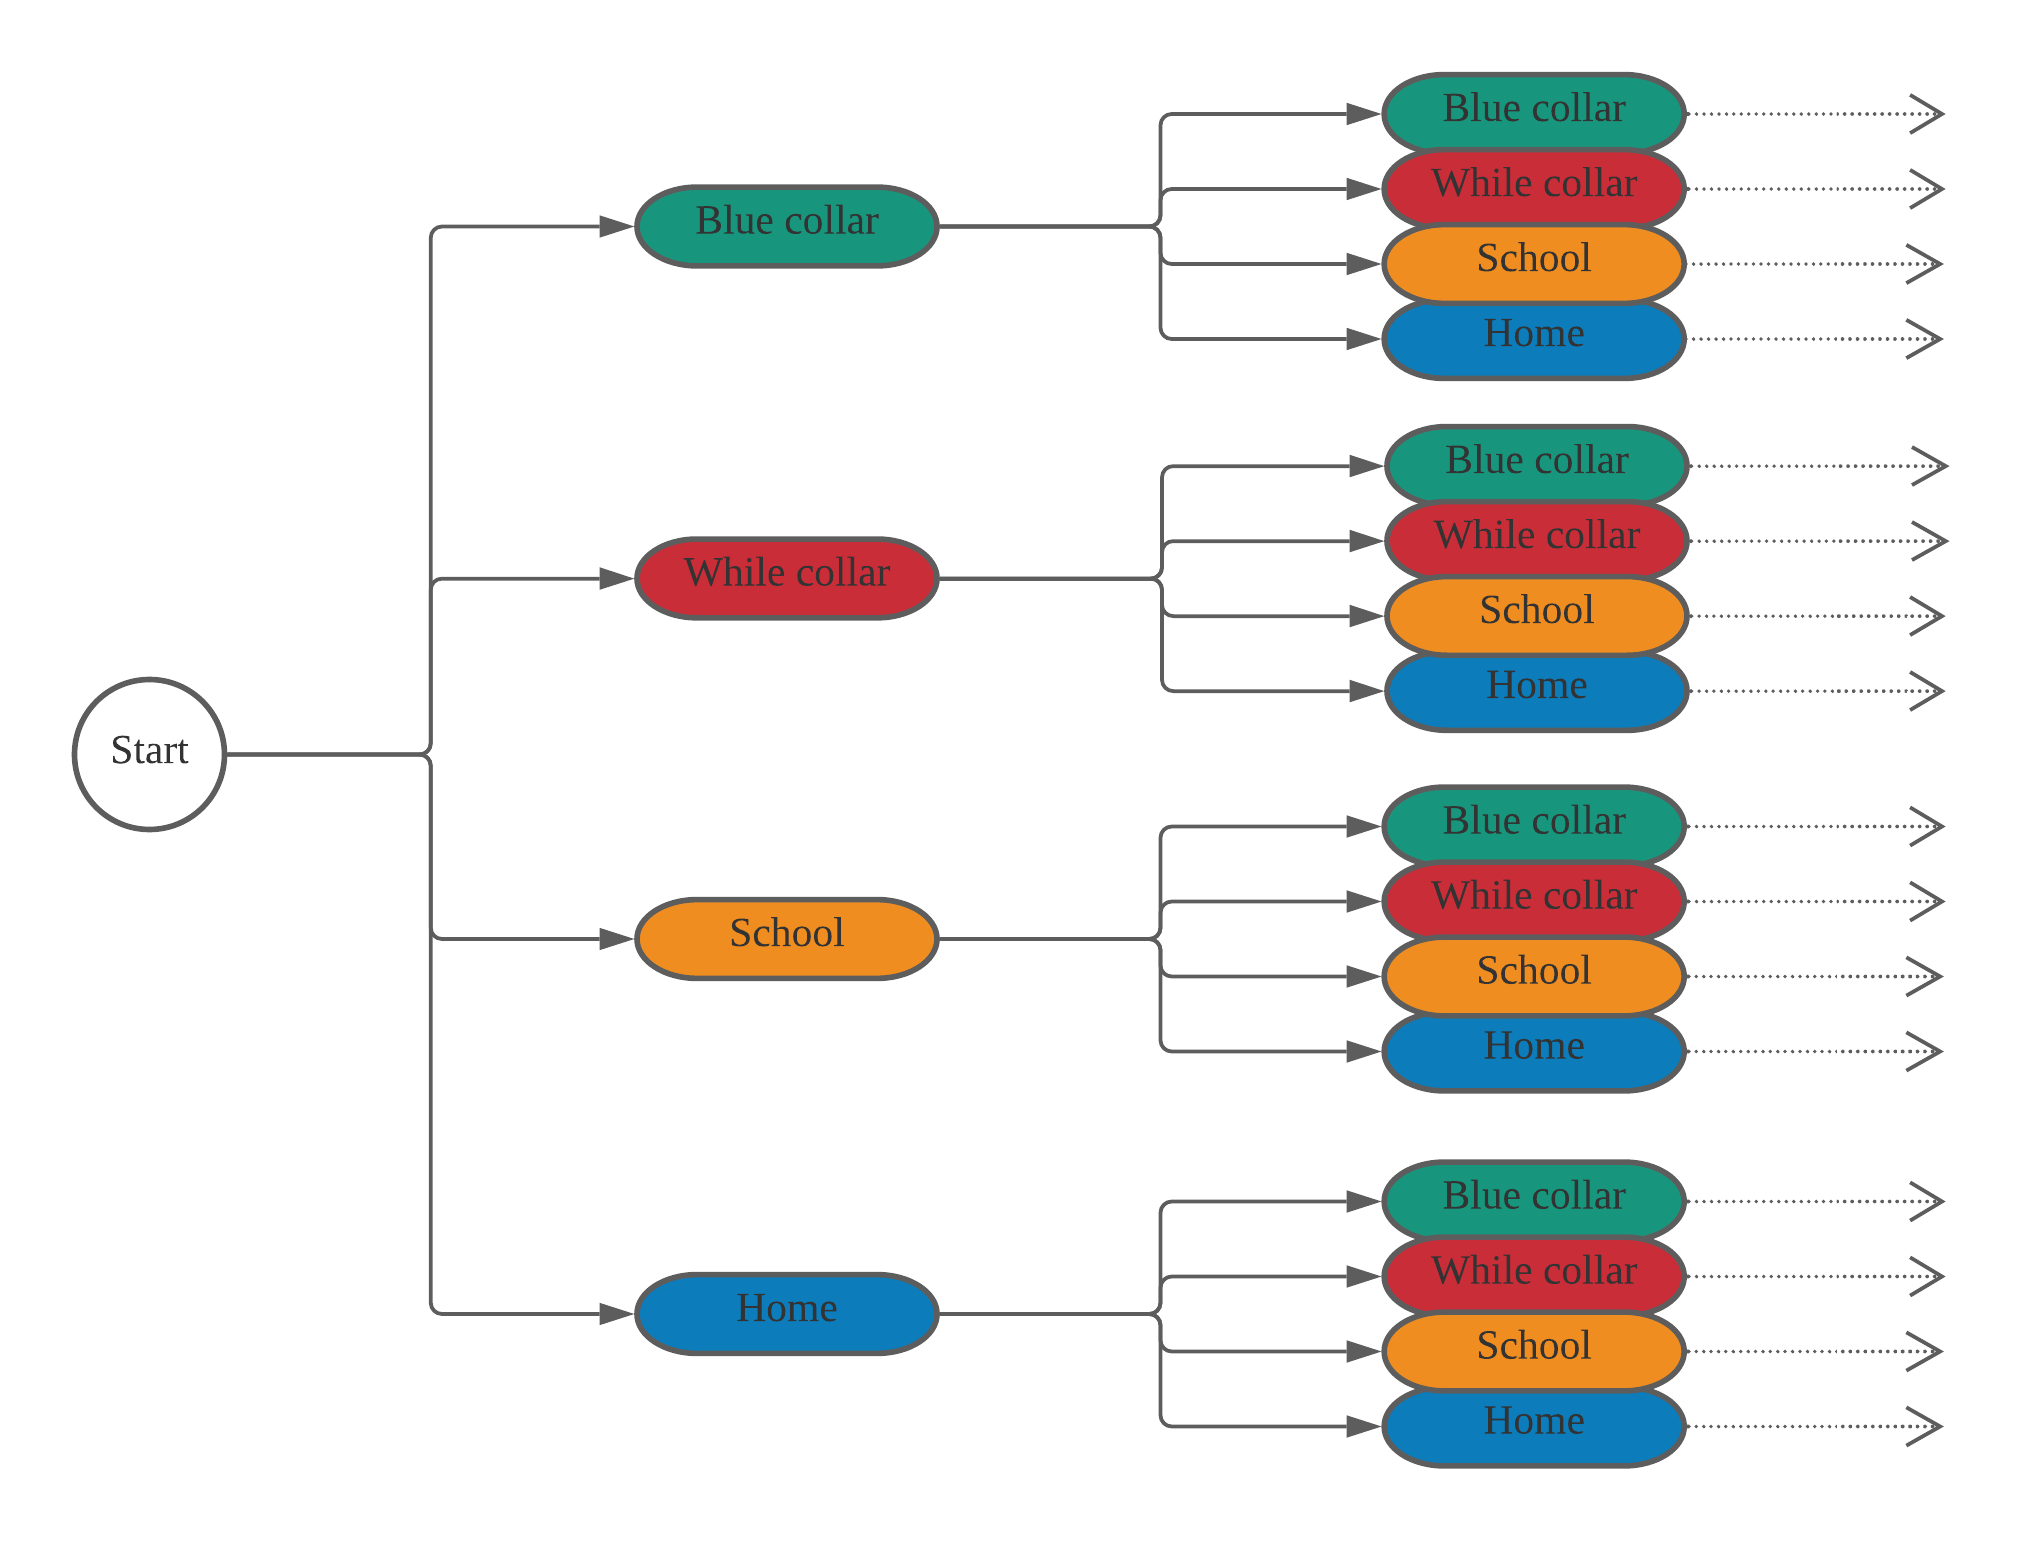
\includegraphics[scale=1]{./resources/kw94-decisiontree}
	\label{fig:corr}
\end{figure}

\vspace{10mm} %5mm vertical space
\begin{figure}[H]
	\caption{Heat map of selective parameters \label{fig:2}}
	\centering
	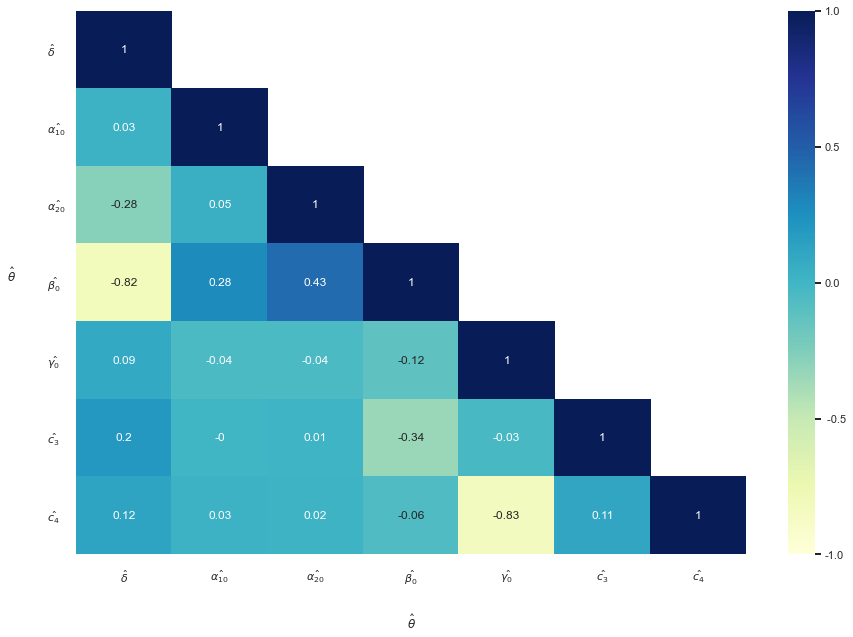
\includegraphics[scale=0.5]{./resources/heatmap}
	\label{fig:corr}
\end{figure}


\vspace{10mm} %5mm vertical space
\begin{figure}[H]
	\caption{ Comparison of shares of occupation decisions over time between scenarios\label{fig:3}}
	\centering
	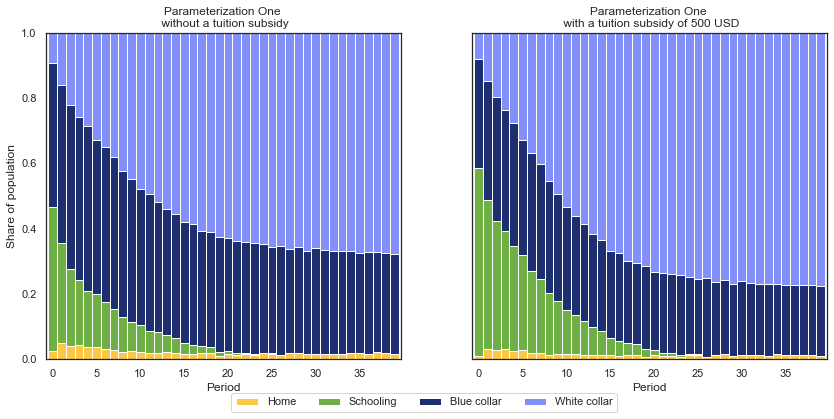
\includegraphics[scale=0.5]{./resources/choiceovertime}
	\label{fig:corr}
\end{figure}

\vspace{10mm} %5mm vertical space
\begin{figure}[H]
	\caption{Probability distribution of QoI\label{fig:4}}
	\centering
	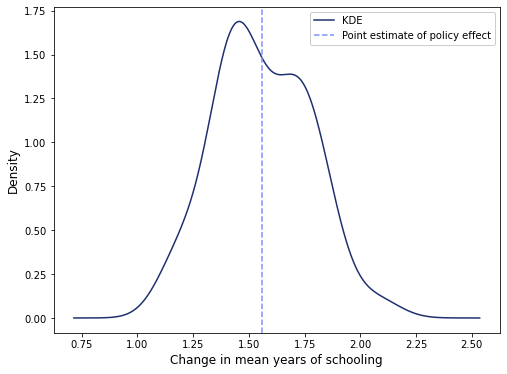
\includegraphics[scale=0.5]{./resources/qoi}
	\label{fig:corr}
\end{figure}


\vspace{10mm} %5mm vertical space
\begin{figure}[H]
	\caption{PDF of output for SA \label{fig:5}}
	\centering
	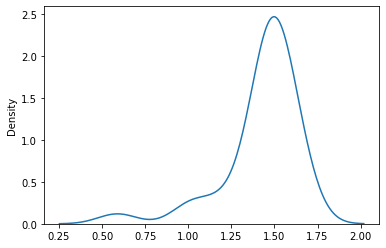
\includegraphics[scale=0.7]{./resources/qoi-SA}
	\label{fig:corr}
\end{figure}


\vspace{10mm} %5mm vertical space
\begin{figure}[H]
	\caption{ Quantile-base sensitivity measures on \cite{keane1994SolutionEstimationDiscrete} model\label{fig:6}}
	\centering
	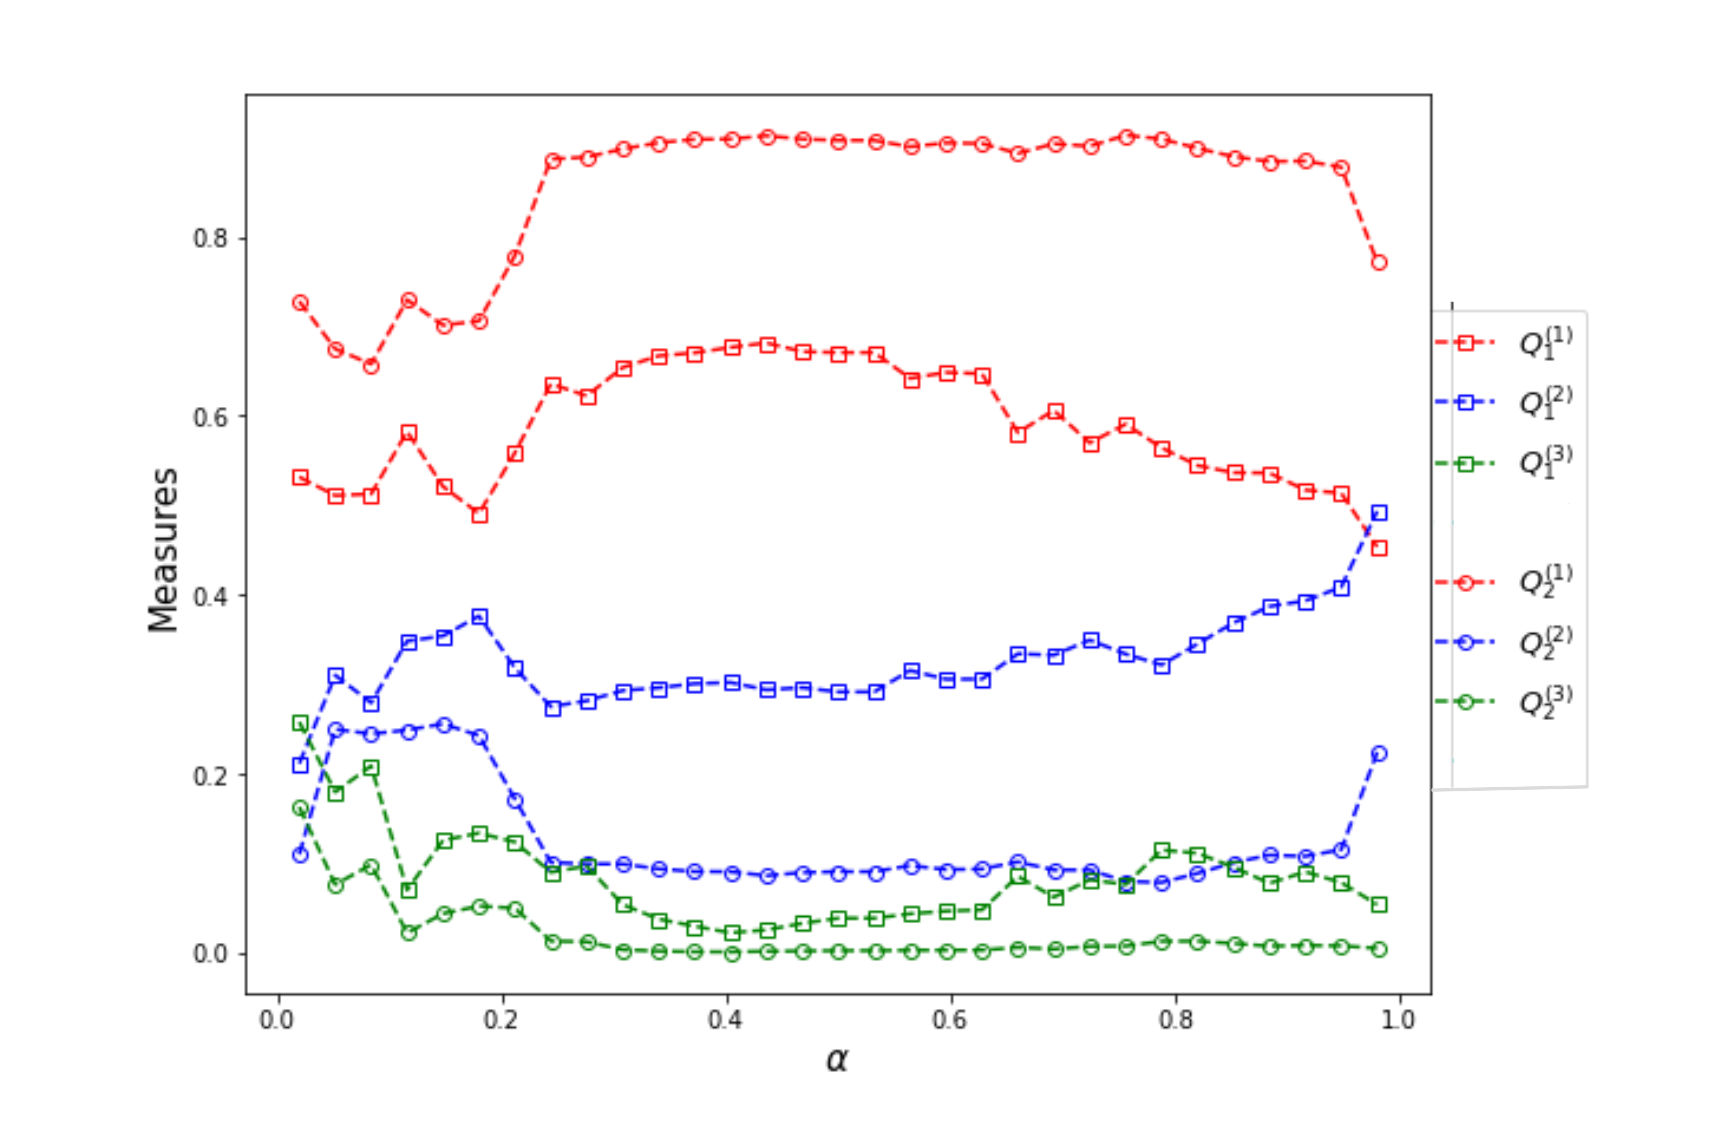
\includegraphics[scale=0.3]{./resources/QBSM}
	\label{fig:corr}
\end{figure}

\newpage
\thispagestyle{empty} % e.g. no page number
\section*{Affidavit}
\vspace*{1.0cm}
"I  hereby confirm that the  work  presented  has  been  performed  and interpreted solely by myself except for where I explicitly identified the contrary. I assure that this work has not been presented in any other form for the fulfillment of any other degree or qualification. Ideas taken from other works in letter and in spirit are identified in every single case."\\
\newline
\newline
\newline

\noindent

\rule{5.5cm}{0.4pt} \phantom{ssssssssssssssssspace} \rule{5.5cm}{0.4pt}\\
\phantom{space}Place, Date \phantom{sssssssssssssssssssssssssssssssssssssssssssspace} Signature




\end{document}

